\chapter{Lebensformen}
\section{Hominini}
Die Zugehörigkeit zu den Hominini wird als hominin bezeichnet. Eine Darstellung der Rassen im Vergleich findet sich in Abb. \ref{fig:allerassen}.
\begin{outline}
	\1 Sämtliche (derzeit bekannte) normale Menschenarten haben sich aus den entsprechenden (gleichen) "Affen" entwickelt. Wesen wie Argonier oder Kajits gibt es bei uns also nicht.
	\1 Die Arten sind immer wie bei der typischen Artenbildung in exklusiven Gebieten entstanden. also es erfolgte eine allgemeine gleiche Entwicklung und manche Arten waren dann abgeschieden von anderen besonderen Umweltbedingungen ausgesetzt und haben deshalb bestimmte Merkmale neu entwickelt oder rückentwickelt
	\1 Die Arten können sich noch mischen, aber wie bei Esel und Pferd (Unterschiede ähnlich wie hier) sind ihre Nachkommen selbst infertil
	\1 die im folgenden vorgestellten Arten sind teilweise nur Anregungen und Beispiele und müssen nicht im Spiel enthalten sein. Ebenso können sie einfach Teil der Welt und unserer Gegend nicht oder nur durch Geschichten bekannt sein. Ist jedoch für später durchaus wichtig :smiley:
	\1 Das heißt auch, dass die Menschenarten keine Federn oder Schuppen haben -- wenn die nicht irgendwie begründbar sind (max. Schuppen). Denn Federn sind was rein von den Vögeln, die mit den Säugern nix zu tun haben
	mit Hörnern bzw. Horn an sich kann natürlich viel gearbeitet werden
	\1 natürlich kann es sein, dass wir durch besondere Umweltgeschehnisse mit viel Magie auch noch andere Arten haben, die sind dann aber "`unnatürlich"'
\end{outline}

\begin{figure}
	\centering
	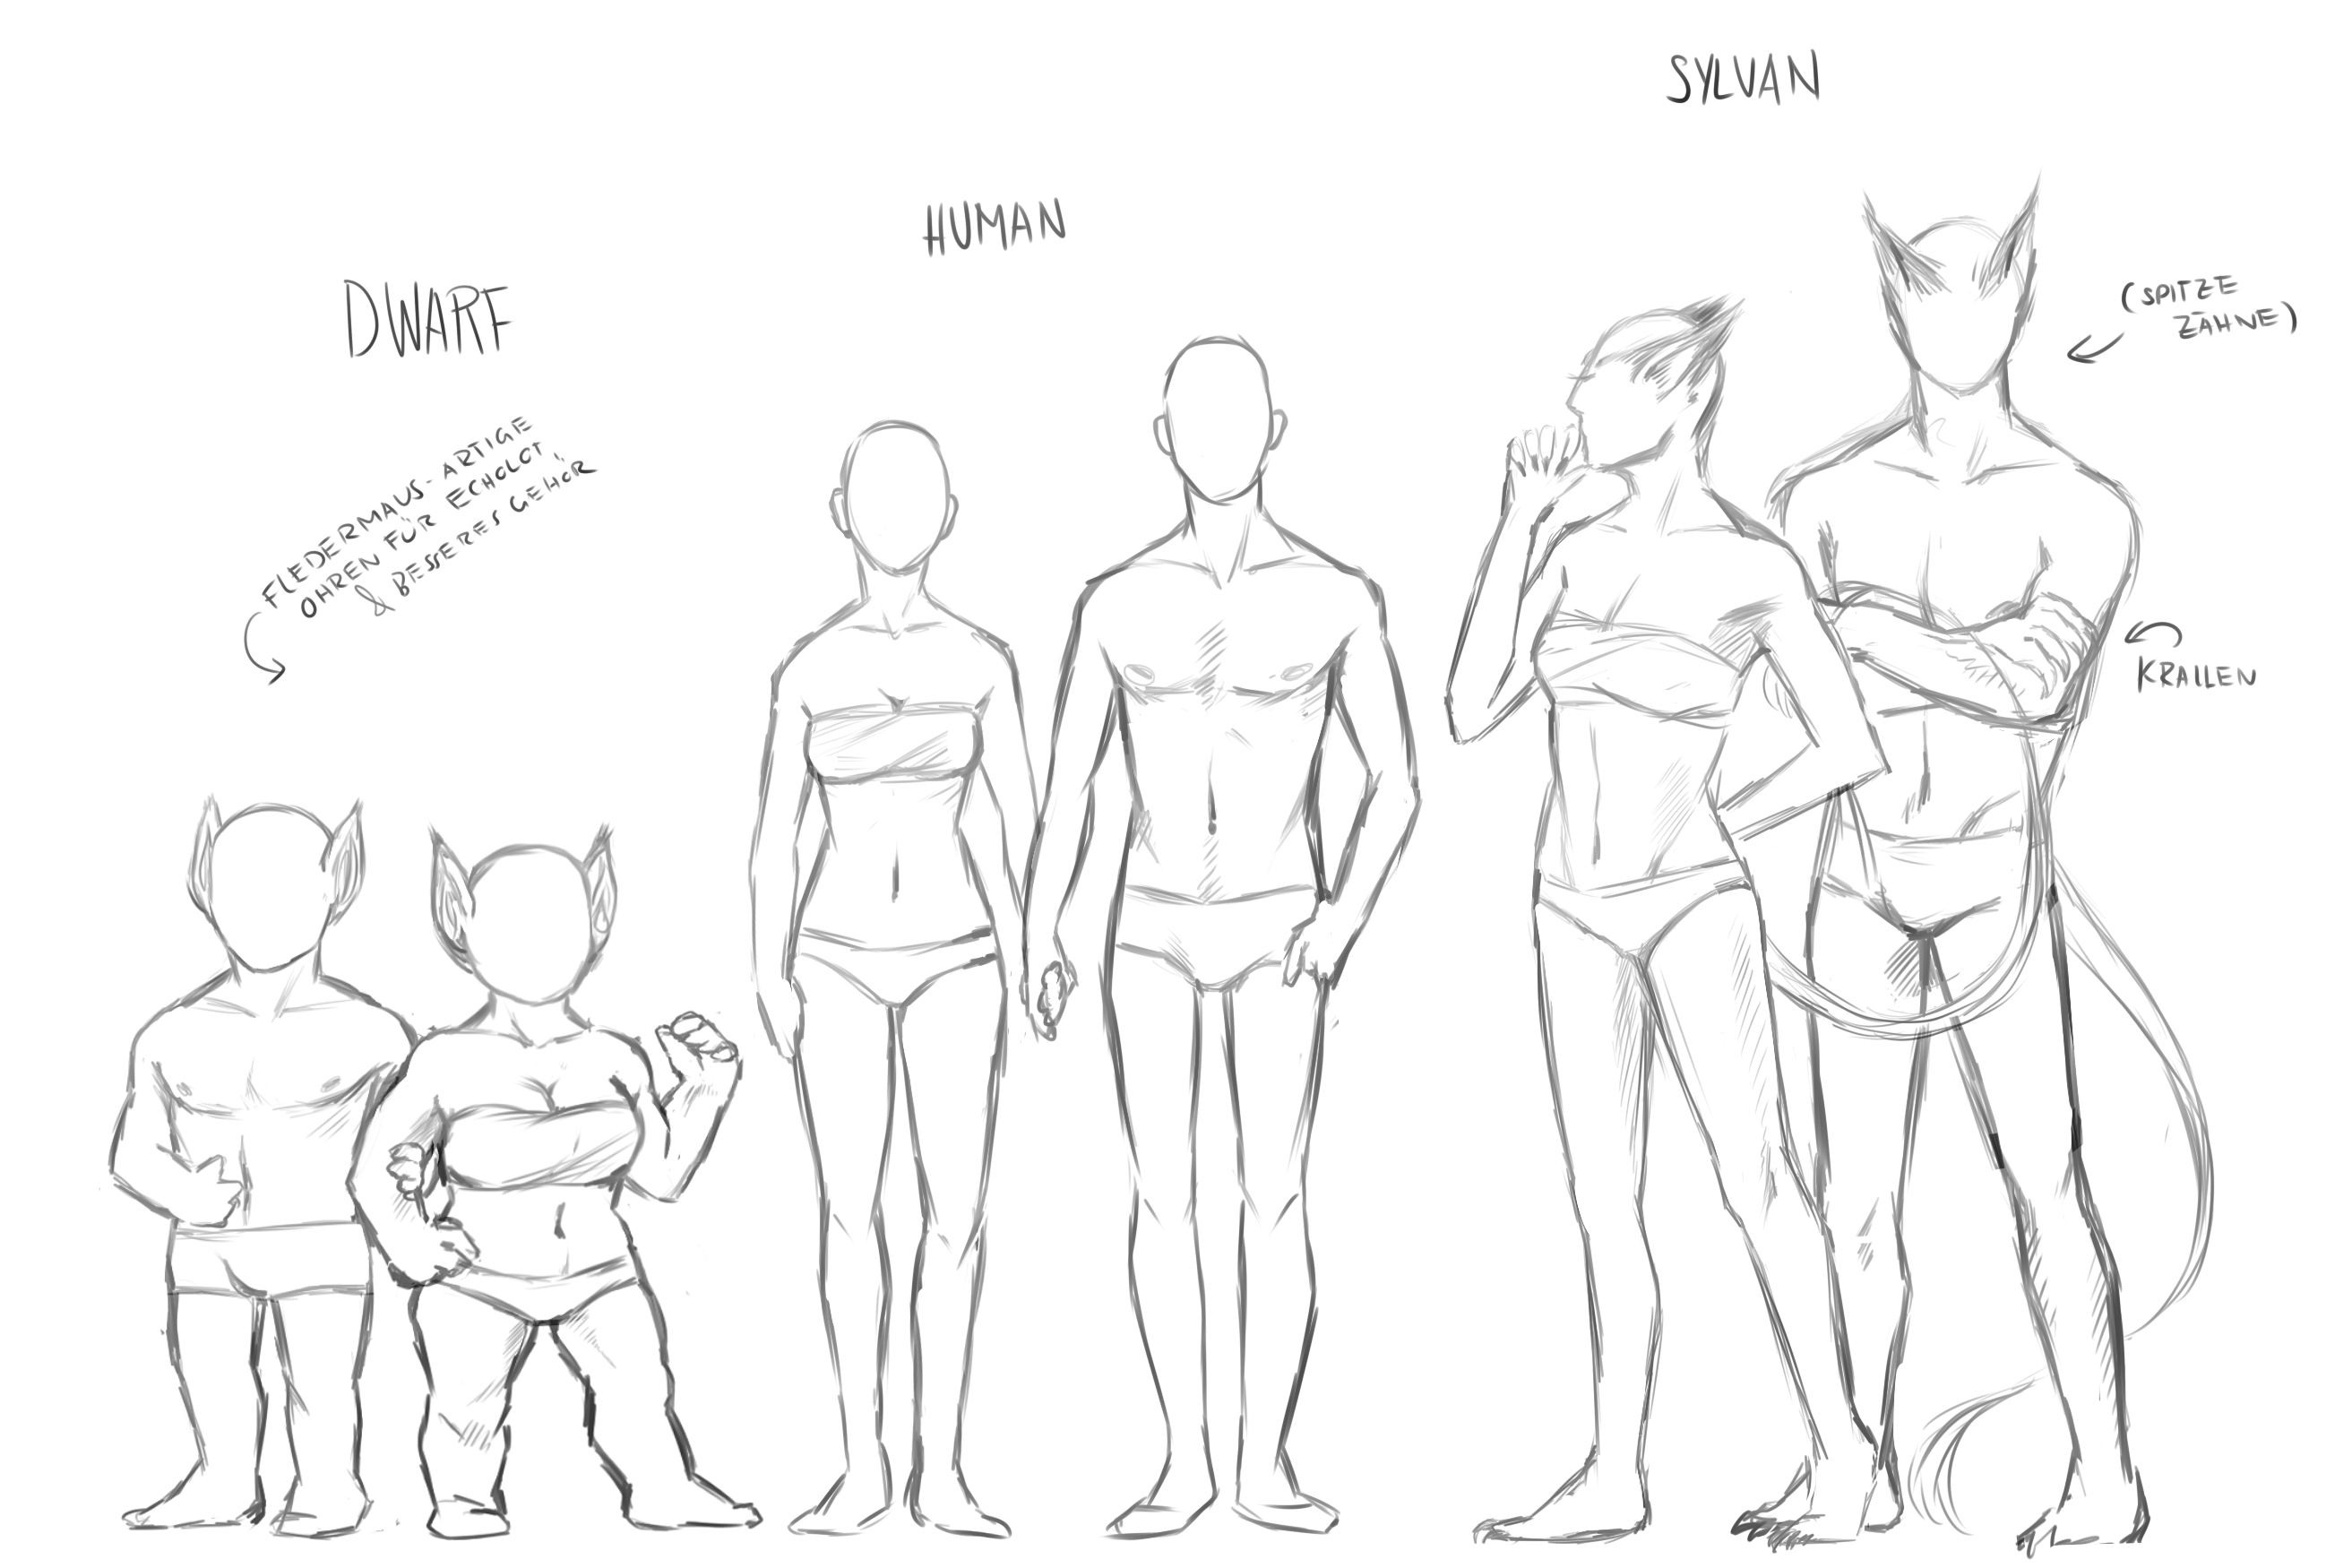
\includegraphics[width=1.0\linewidth]{Abbildungen/Weltenbau/Lebensformen/allerassen}
	\caption{Vergleich der unterschiedlichen homininen Rassen.}
	\label{fig:allerassen}
\end{figure}


\paragraph{Stammbaum} Hier soll man später den Stammbaum der Hominini finden können. Also welche Art sich wann von welcher anderen abgezweigt hat.

\paragraph{Besonderheiten}
Einige Humanoide haben gemeinsame Besonderheiten im Vgl. zu den RL-Menschen. Dies hängt immer davon ab, wann sich die jeweiligen Arten voneinander abgespalten haben. \\
So haben z.B. alle Humanoiden ein besonderes Sinnesorgan (siehe Standard bei Menschen, Besonderheiten bei der jeweiligen Art erwähnt).


\subsection{Vorwissen}
Bei der Erstellung der Rassen bitte folgende Punkte (aus \href{https://de.m.wikipedia.org/wiki/Primaten#Merkmale}{Wikipedia}) beachten:\\
Obwohl die Primaten eine relativ klar definierte Säugetierordnung sind, gibt es relativ wenig Merkmale, die bei allen Tieren dieser Ordnung und sonst bei keinem anderen Säugetier zu finden sind. Dennoch lassen sich laut dem Biologen Robert Martin neun Merkmale der Primatenordnung festhalten:
\begin{itemize}
	\item Der große Zeh ist opponierbar (Ausnahme: Mensch) und die Hände sind zum Greifen geeignet.
	\item Die Nägel an den Händen und Füßen der meisten Arten sind flach (keine Krallen). Zudem haben Primaten Fingerabdrücke.
	\item Die Fortbewegung ist von den Hinterbeinen dominiert, der Schwerpunkt liegt näher an den hinteren Gliedmaßen.
	\item Die olfaktorische Wahrnehmung ist unspezialisiert und bei tagaktiven Primaten reduziert.
	\item Die visuelle Wahrnehmung ist hochentwickelt. Die Augen sind groß und nach vorne gerichtet (Stereoskopie).
	\item Die Weibchen haben geringe Wurfgrößen. Schwangerschaft und Abstillen dauern länger als bei anderen Säugetieren vergleichbarer Größe.
	\item Die Gehirne sind verhältnismäßig größer als bei anderen Säugetieren und weisen einige einzigartige anatomische Merkmale auf.
	\item Die Backenzähne sind relativ unspezialisiert und es gibt maximal drei; sowie maximal zwei Schneidezähne, einen Eckzahn, und drei Prämolare.
	\item Es gibt weitere (für Systematiker nützliche) subtile anatomische Besonderheiten, die sich jedoch nur schwer funktionell einordnen lassen.
	\item \textbf{Körpergröße:} Einige Arten haben einen ausgeprägten Geschlechtsdimorphismus, wobei die Männchen mancher Arten doppelt so schwer wie die Weibchen sein können und sich auch in der Fellfarbe unterscheiden können. 
	\item \textbf{Behaarung:} Der Körper der meisten Primaten ist mit Fell bedeckt, dessen Färbung von weiß über grau bis zu braun und schwarz variieren kann. Die Handflächen und Fußsohlen sind meistens unbehaart, bei manchen Arten auch das Gesicht oder der ganze Kopf (zum Beispiel Uakaris). Am wenigsten behaart ist der Mensch. 
	\item \textbf{Augen:} Die größten Augen aller Primaten haben die Koboldmakis. Bei den größtenteils nachtaktiven Feuchtnasenprimaten ist zusätzlich eine lichtreflektierende Schicht hinter der Netzhaut, das Tapetum lucidum vorhanden.
	\item \textbf{Nase:} Namensgebender Unterschied der beiden Unterordnungen ist der Nasenspiegel (Rhinarium), der bei den Feuchtnasenprimaten feucht und drüsenreich ist und sich in einem gut entwickelten Geruchssinn widerspiegelt. Die Trockennasenprimaten hingegen besitzen einfache, trockene Nüstern und ihr Geruchssinn ist weit weniger gut entwickelt. 
	\item \textbf{Zähne:} Die Form insbesondere der Backenzähne gibt Aufschluss über die Ernährung. Vorwiegend fruchtfressende Arten haben abgerundete, insektenfressende Arten haben auffallend spitze Molaren. Bei Blätterfressern haben die Backenzähne scharfe Kanten, die zur Zerkleinerung der harten Blätter dienen. 
	\item \textbf{Schwanz:} Für viele baumbewohnende Säugetiere ist ein langer Schwanz ein wichtiges Gleichgewichts- und Balanceorgan, so auch bei den meisten Primaten. Jedoch kann der Schwanz rückgebildet sein oder ganz fehlen. Mit Ausnahme der Menschenartigen, die generell schwanzlos sind, ist die Schwanzlänge kein Verwandtschaftsmerkmal, da Stummelschwänze bei zahlreichen Arten unabhängig von der Entwicklung vorkommen. Sogar innerhalb einer Gattung, der Makaken, gibt es schwanzlose Arten (zum Beispiel der Berberaffe) und Arten, deren Schwanz länger als der Körper ist (zum Beispiel der Javaneraffe). Einen Greifschwanz haben nur einige Gattungen der Neuweltaffen ausgebildet (die Klammerschwanzaffen und die Brüllaffen). Dieser ist an der Unterseite unbehaart und mit sensiblen Nervenzellen ausgestattet.
	\item \textbf{Aktivitätszeiten:} Die unterschiedlichen Aktivitätszeiten haben sich auch im Körperbau niedergeschlagen, so sind in beiden Untergruppen nachtaktive Tiere durchschnittlich kleiner als tagaktive. Eine weitere Anpassung an die Nachtaktivität stellt der bessere Geruchssinn der Feuchtnasenprimaten dar. Vergleichbar mit anderen Säugetieren ist die Tatsache, dass Arten, die sich vorwiegend von Blättern ernähren, längere Ruhezeiten einlegen, um den niedrigen Nährwert ihrer Nahrung zu kompensieren. 
\end{itemize}


\subsection{Menschen} \label{rasse:mensch}
\begin{outline}
	\1 sehen an sich wie Menschen aus. Durchschnittliche Körpergröße: 165 cm für Frauen, 180 vm für Männer
	\1 zusätzliches Sinnesorgan zum Spüren von Magie. Dieses funktioniert ähnlich wie das Seitenlinienorgan der Fische. Öffnungen am Hals links und rechts erlauben die Wahrnehmung von Magie bzw. deren Intensität. Man kann sie spüren wie Druck. Siehe auch Abb. \ref{fig:sinnesorganauswahl}.
\end{outline}

\begin{figure}
	\centering
	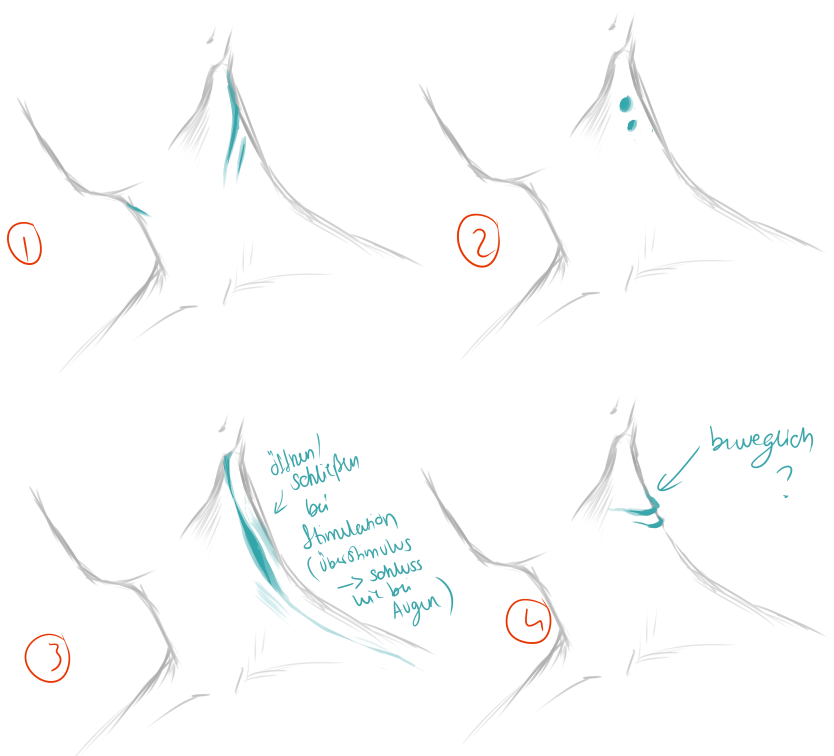
\includegraphics[width=0.7\linewidth]{Abbildungen/Weltenbau/Lebensformen/Sinnesorgan_Auswahl}
	\caption{Die möglichen Formen eines Sinnesorgans zum Spüren von Magie.}
	\label{fig:sinnesorganauswahl}
\end{figure}

\subsection{Dunkles Volk}

\subsection{Zwerge} \label{rasse:zwerg}
\begin{outline}
	\1  Zwerge sind "kleine", stämmige Menschen (da solche durch Tunnel besser hindurch kommen) mit einer Körpergröße von durchschnittlich 1,25 m bei Frauen und 1,35 m bei Männern. Dabei sind die Gräbern sehr Kräftige aufgrund der anstrengenden körperlichen Arbeit, wie in Abb. \ref{fig:zwerggraeber} zu sehen ist. Die restlichen sind wie Menschen unterschiedlichen Körperbaus, zu sehen in Abb. \ref{fig:zwergkaufmann} und\ref{fig:zwerghaendlerin}. Ihr Körper ist bezgl Kopf und Torso vergleichbar mit Menschen, doch ihre Gliedmaßen scheinen verkürzt.
	\1 leben in Höhlensystemen die tief unter die Oberfläche reichen
	\1 ihre \textbf{Sicht} ist nicht so gut, da das im Allgemeinen recht unwichtig unter der Erde ist
	\1 dafür ist ihr \textbf{Gehör} extrem gut. Zudem können sie (ähnlich wie Fledermäuse) auch höhere und tiefere Schwingungen wahrnehmen und sie zur Orientierung nutzen. Sie haben zwar kein Organ, um diese Schallwellen so auszustoßen, allerdings zeigt sich das in ihrer Magie. Ihre Ohren sind dadurch etwas abstehender und deutlich beweglicher (ähnlich mehrere Tiere, zB auch Fledermäuse)
	\1 auch ihr \textbf{Geruch} ist verbessert: mit diesem können sie schnell gefährliche Dämpfe wahrnehmen oder Beutetiere unter der Erde riechen.
	\1 Magie-bezogen hat sich bei ihnen nämlich hauptsächlich die \textbf{\npref{sec:vibrationsmagie} (änderbar)} durchgesetzt: damit können sie die Schwingungen in der Luft erzeugen, die sie mit ihrem feinen Gehör auswerten und sich so auch im Dunklen zurechtfinden können. Weiterhin nützt ihnen die Vibration beim Tunnelbau sehr viel
	\1 weiterhin hat sich ihre \textbf{Sauerstoffverwertung} angepasst: sie sind in der Lage, schon geringe Mengen Sauerstoff in der Umgebungsluft effektiv zu nutzen und somit auch tief unter der Erde vernünftig atmen zu können. Diese erhöhte Verwertbarkeit ist ein gradueller Anpassungsprozess, der nicht von jetzt auf gleich funktioniert. Das ist vor allem beim Aufstieg aus den Tiefen relevant, denn wenn sie zu schnell an die Oberfläche mit ihrer hohen Sauerstoffkonzentration kommen, dann erleiden sie Symptome wie bei der Hyperventilation und sterben. Daher müssen sie die ersten Stunden bis Tage eine Art Maske/Sack mit sich herum tragen, mit der sie sich graduell an die höhere Konzentration gewöhnen können. Weiterhin beschleunigt die hohe O2-Konzentration ihre Zellalterung und somit ihren Tod. Dies führt dazu, dass sie sich auf der Oberfläche kaum finden lassen  und vorrangig mehrere Meter tief unter der Erde wohnen.
\end{outline}

\begin{figure}
	\centering
	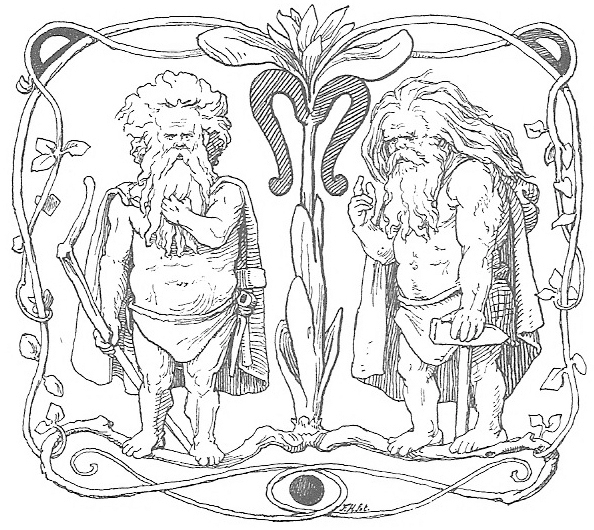
\includegraphics[width=0.7\linewidth]{Abbildungen/Weltenbau/Lebensformen/ZwergGraeber.png}
	\caption{Typische Gräber der Zwerge.}
	\label{fig:zwerggraeber}
\end{figure}

\begin{figure}
	\begin{minipage}{0.49\textwidth}
		\centering
		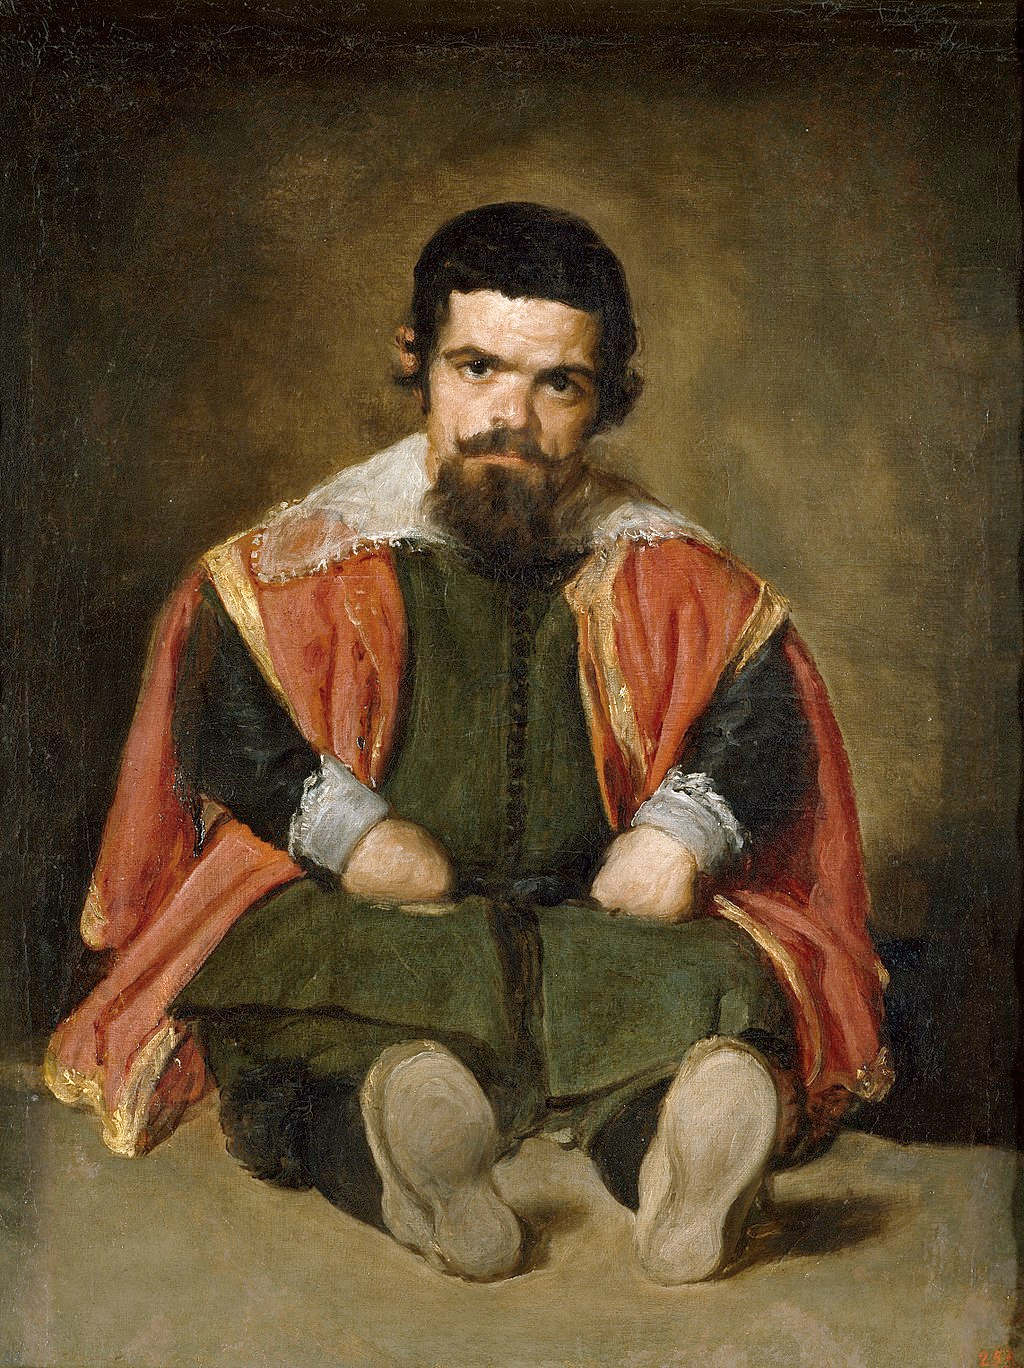
\includegraphics[width=0.8\linewidth]{Abbildungen/Weltenbau/Lebensformen/ZwergKaufmann.png}
		\caption{Ein zwergischer Kaufmann.}
		\label{fig:zwergkaufmann}
	\end{minipage}
	\hfill
	\begin{minipage}{0.49\textwidth}
		\centering
		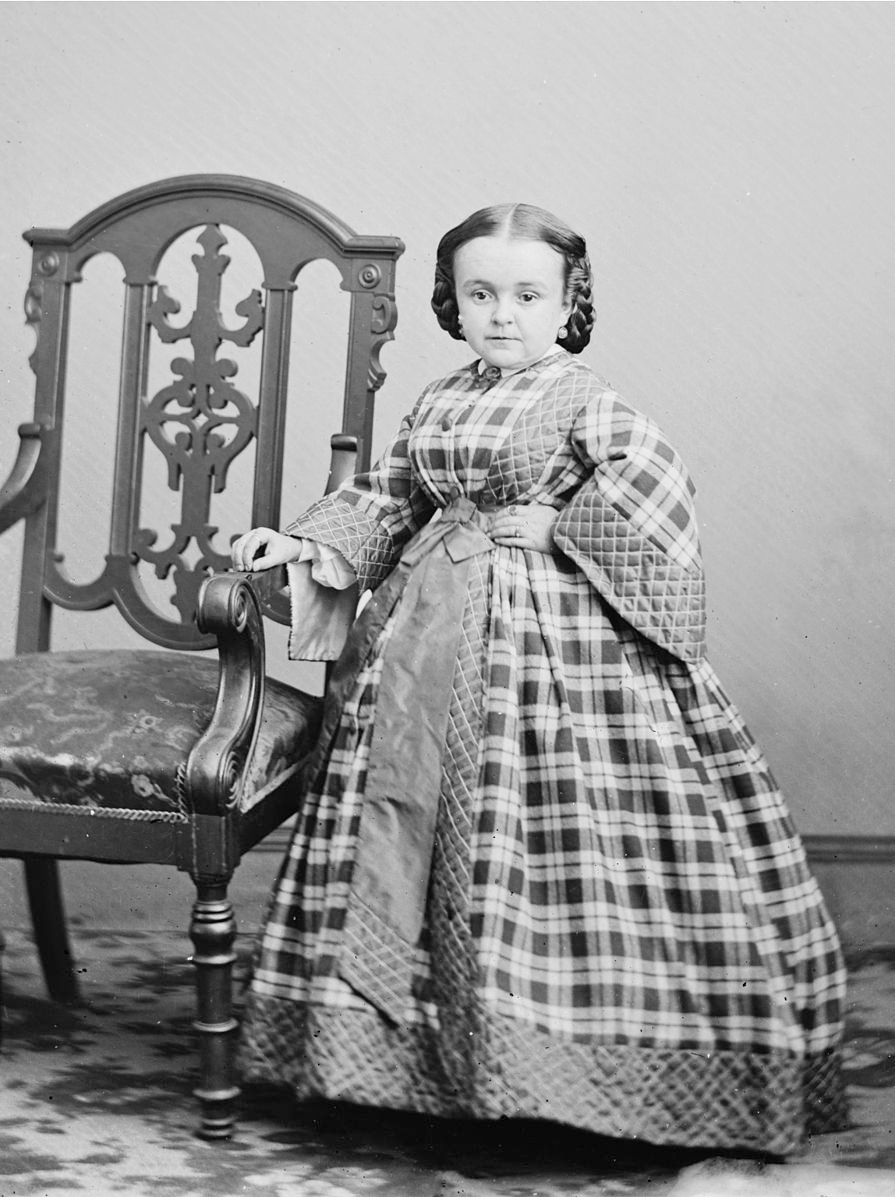
\includegraphics[width=0.8\linewidth]{Abbildungen/Weltenbau/Lebensformen/ZwergHaendlerin.png}
		\caption{Eine zwergische Händlerin.}
		\label{fig:zwerghaendlerin}
	\end{minipage}
\end{figure}



\subsubsection{Entstehung}
Die Vorfahren der Zwerge, eine Menschenaffenart normaler Größe, sind eine Gruppe, die sich in einer Gegend niedergelassen hatten, die einen gefährlichen größeren Jäger hatte. Das zwang diese Menschen dazu, sich in die natürlichen Höhlen der Gegend zurück zu ziehen. Die Jagd bei Nacht wurde bevorzugt, da es tagsüber gefährlicher war. Über die Zeit hinweg passten sie sich ihren Bedingungen an: Leben hauptsächlich im Dunklen und unter der Erde, draußen nur nachts. Für eine wachsende Gemeinschaft schließlich mussten immer tiefere Höhlen gegraben werden und so... kam es zur Entwicklung der Rasse der Zwerge, wie es sie heute gibt



\subsection{Halblinge} \label{rasse:halbling}
Ziemlich genau \href{https://de.wikipedia.org/wiki/Pygm\%C3\%A4en}{Pygmäen}.


\subsection{Sylvan} \label{rasse:sylvan}
ein Sylvan, mehrere Sylvaner
\begin{outline}
	\1 diese Menschenart lebt in dem \npref{formation:gigantus}, wo die Bäume so hoch werden, dass wir im Vgl. so groß wie Mäuse oder Käfer sind
	\1 Sie leben auf den Ebenen über dem Boden, wo die riesigen Äste der Bäume neue Ebenen erschaffen. Seltenst betreten sie den Waldboden
	\1 Ich stelle sie mir allerdings auch nicht am Ast schwingend vor, schon als Baumbewohner wie Menschen sie werden würden, also Natur unterwerfend und nutzen.
	\1 aufgrund des extremen Vorteils der Fähigkeit, Druck bzw Wind zu beeinflussen, ebenso wie die Atombindungen zu verhärten; aufgrund dessen haben diese Allele alle anderen verdrängt und man findet bei dieser Menschenart keine andere Magienutzung mehr
\end{outline}

\subsubsection{Aussehen der Sylvaner}
\begin{outline}
	\1 sie sind etwas größer als normale Menschen (Durchschnitt 15 cm größer: Frauen 180 cm, Männer 195 cm), deutlich dünner und bewegen sich sehr grazil
	\1 eine ihrer Anpassungen an den Lebensraum: der \textbf{Schwanz}. Sie haben den Schwanz wieder rückentwickelt, weil der sehr stark bei der Stabilisation des Gleichgewichts hilft, was in den luftigen Höhen des Lebensraums von starkem Vorteil ist
	\1 keine \textbf{Krallen} (sie sollen nicht zu sehr zu Mensch+Katze oder Fuchs werden). Zudem: wozu brauchen sie diese? Sie behindern beim benutzen von Werkzeugen. Vllt ein paar längere Finger oder größere Hände, im Verhältnis. 
	\1 \textbf{Behaarung}. Wir möchten ungerne, dass ihnen die Menschlichkeit zu sehr abhanden kommt und sie zu sehr „Monster“ werden. Also lange Haare am ganzen Körper wären komisch. Kurze Haare, so 0,5-2 cm in der Variation plus Kopfbehaarung halte ich für sinnvoll. Denn wir stellen da ja praktisch eine leichte Rückentwicklung mehrere Merkmale dar. Also auch Haupthaar. Hände und Füße sollten nackt sein. Das Gesicht großteils auch, dafür läuft ihre Haarlinie bis zu inklusive den Augenbrauen runter (kürzere Haare auf der Stirn, keine extra Augenbrauen) und seitlich stärker auf die Wangen rauf.\\
	Idee: Sie haben einen farblichen Fellwechsel zwischen Sommer und Winter
	\1 ggf. sind die \textbf{Augen} größer (Diskussion)
	\1 \textbf{Ohren}: keine spezielle Anpassung, also normale menschliche Ohren
\end{outline}

\subsubsection{Entstehung}
Geschichtlich sollten sich die Sylvans recht früh von den Urmenschen abgespalten haben.

\subsubsection{Kultur}
\begin{outline}
	\1 ein Ritual könnte sein, dass sie die Leichen der Toten in Ast- und Blattwiegen aufbahren und sie dann  Richtung Erdboden schicken
\end{outline}





\subsection{Unda} \label{rasse:unda}
ein Unda, mehrere Undar
\begin{outline}
	\1 diese Art lebt am Rande bzw. halb in großen Gewässern
	\1 \textbf{Sonar:} In Zusammenhang mit Magie und Körperlichem haben die Undar ein präzises Biosonar entwickelt: sie können mittels Magie hochfrequentige Wellen erzeugen, mit denen sie ihre Umgebung ähnlich wie Fledermäuse abtasten. Um den Schall präzise zu interpretieren, haben sie große bewegliche Ohren. Zudem können sie mit ihrer Magie lauten Schall erzeugen, was sie gut bei der Jagd zur Betäubung einsetzen. 
\end{outline}

\subsubsection{Körperliches}
\begin{outline}
	\1 bei ihnen entwickeln sich die Schwimmhäute an den \textbf{Händen} während der Embryonalentwicklung nicht mehr zurück; zudem haben sie vergleichsweise große und längliche \textbf{Füße} entwickelt
	\1 Eine \textbf{dicke Fettschicht} schützt sie vor der Kälte des Wassers: Kaltes Wasser entzieht dem Körper wesentlich mehr Wärme als Luft. Undar müssen aber, wie die meisten anderen Säugetiere, eine konstante Temperatur von 36 bis 37 Grad Celsius halten, da sonst das Herz-Kreislauf-System versagt.
	\1 Da Wasser viel dichter als Luft ist, fällt die Bewegung darin entsprechend schwerer. Mit einem ganz speziellen Trick setzen sie ihn herab: An der glatten weichen Haut würden sich beim Schwimmen normalerweise Turbulenzen bilden. Diese Verwirbelungen erhöhen den Wasserwiderstand und würden sie mit ihrer großen \textbf{Körperoberfläche} stark abbremsen. Aber Undar sind in der Lage, die entstehenden Wirbel mit Drucksensoren zu ertasten und durch feine Hautrillen auszugleichen.
	\1 Da sie unter Wasser nicht atmen können, haben die Undar ihren Sauerstoffhaushalt an das Leben unter Wasser angepasst. Mit einem Atemzug können sie 80 bis 90 Prozent ihrer \textbf{Atemluft} austauschen. Beim Menschen sind es gerade einmal zehn bis 15 Prozent. Damit ihnen auf längeren Tauchgängen nicht die Luft ausgeht, können sie den Sauerstoff viel besser speichern: ihr Blut ist stärker mit Hämoglobin angereichert und sie können mehr Sauerstoff in den Muskeln zwischenspeichern. Das gesamte System der Energiegewinnung ist äußerst effizient.
	\1 \textbf{Sinne:} Die meisten Wale besitzen, ähnlich wie viele andere Säugetiere, auch gut ausgebildete \textbf{Augen}. Da die Sichtverhältnisse im Wasser jedoch wesentlich schlechter sind als an Land, haben sich die Undar im Laufe ihrer Entwicklung auf andere Sinne spezialisiert, besonders auf das \textbf{Hören} und \textbf{Tasten}. Das \textbf{Riechen} ist eher unterentwickelt.
\end{outline}

\subsubsection{Entstehung}
...


\subsection{Ferus} \label{rasse:ferus}
ein Ferus, mehrere Feri
\begin{outline}
	\1 ...
\end{outline}

\subsubsection{Körperliches}
\begin{outline}
	\1 ...
\end{outline}

\subsubsection{Entstehung}
...



\section{Tiere}
\subsection{Echte Tiere}
\paragraph{Regenbogen Oktopus} Könnte tatsächlich eine Inspiration für Meerjungfrauen gewesen sein (insbes. Start des Videos): \href{https://img-9gag-fun.9cache.com/photo/aVYpQVK\_460svvp9.webm}{9gag.com}
\paragraph{Axolotl} Sind einfach süß. Wir wollen sie dabei haben!

\section{Pflanzen}
\subsection{Echte Pflanzen}
\paragraph{Sandbüchsenbaum} \href{https://de.wikipedia.org/wiki/Sandb\%C3\%BCchsenbaum}{Wikipedia}. Die Stacheln des Baumes sind voller Gift. Die Früchte sehen wie kleine Kürbisse aus und wenn sie reif sind, explodieren sie und schleudern die Samen mit bis zu 240 km/h weg.

\section{Mikroorganismen}
